\chapter{\label{ch:1-intro}Introduction} 

%\minitoc


%% To do:
% MM MGUS SMM immune paper

\section{Overview}
Multiple myeloma (MM) is an incurable cancer of plasma cells.
MM accounts for 1-2\% of all cancers and 10\% of all hematological malignancies\cite{international2003criteria}.
In 2020, it was estimated that the total worldwide incidence of MM was 160,000\cite{ludwig2020multiple}.
Over the last two decades, several classes of drugs have been approved for treatment in MM, including proteasome inhibitors (PIs), immunomodulatory imide drugs (IMiDs) and monoclonal antibodies.
These are now standard drugs in the treatment of MM, and subsequently a drastic improvement in survival rates has been seen--- median survival time for newly diagnosed MM patients has almost doubled in the last 10 years\cite{kazandjian2016look}.
However, MM still remains an incurable disease, with patients eventually relapsing and becoming resistant to drugs they have previously been treated with.
Drug resistance is one of the biggest barriers in the treatment of MM\@.
Therefore, the generation of novel compounds effective against MM is important to extend progression-free survival of patients and work towards finding a cure to MM\@.
This thesis aims to identify novel drugs effective against MM, which are capable of overcoming drug resistance to conventional MM therapies.
It also aims to characterise the transcriptional landscape of MM, following treatment with these novel compounds, to ascertain the mechanism of action in MM and identify any potential side effects of treatment.
MM is a heterogeneous disease with prominent interactions with the surrounding immune microenvironment.
Therefore, MM cells must be examined at the single-level along with other cells residing in the bone marrow niche, to fully capture the heterogeneity and immune interactions we see in myeloma.

This introduction will give a brief overview of the immune system, multiple myeloma (MM), and current MM treatments.
The genome, epigenome, transcriptome and proteome will be introduced, followed by a review of the technological advancements and informatics tools used to decode them.
Chapter 2 introduces the enzyme class: aminoacyl tRNA synthetases (aaRS) and reviews literature regarding their role in disease and the application of therapeutics targeting enzymes in this class.
Next, literature surrounding the drug halofuginone, a Prolyl-tRNA synthetase (ProRS) inhibitor, is reviewed and its application in MM is considered.

% 1
\section{The immune system}
This thesis employs multi-omics techniques to assess the effectiveness and mechanism of action of novel therapeutics in multiple myeloma.
MM is a cancer of terminally differentiated B lymphocytes (a type of white blood cell which acts as part of the adaptive immune system to fight infection).
In chapter \ref{ch:6-sc} single-cell RNA-sequencing is applied to MM bone marrow samples and the different cellular components of the immune system are discussed.
Therefore, a brief introduction will be given into the different facets of the immune system.

\subsection{The function of the immune system}
Humans are exposed to millions of potential pathogens every day and would die without defences to be able to protect themselves from infection.
These defences can be innate or adaptive.
An example of an innate defence is the skin acting as a physical barrier between the outside world and the body.
Innate responses are non-specific and relied upon as the first line of defence, however sometimes a more sophisticated, specialised response is required-- called the adaptive immune response\cite{alberts2007molecularimmune}.
%Another example of an innate defence is non-specific engulfing (phagocytosis) of foreign pathogens by macrophages (a type of white blood cell).
Both innate and adaptive immune responses rely on cells produced by the hematopoietic system.
Hematopoiesis is the process in which the body produces blood\cite{alberts2007molecularstem}.
Postnatally, the major hematopoietic organs are bone marrow, lymph nodes, the spleen and the thymus.

\subsection{Hematopoietic stem cell differentiation}
All blood cells originate from multipotent hematopoietic stem cells (HSCs), located in the bone marrow (BM).
%
%%%
%% Immune cell figure
\begin{figure}[htb]
\centering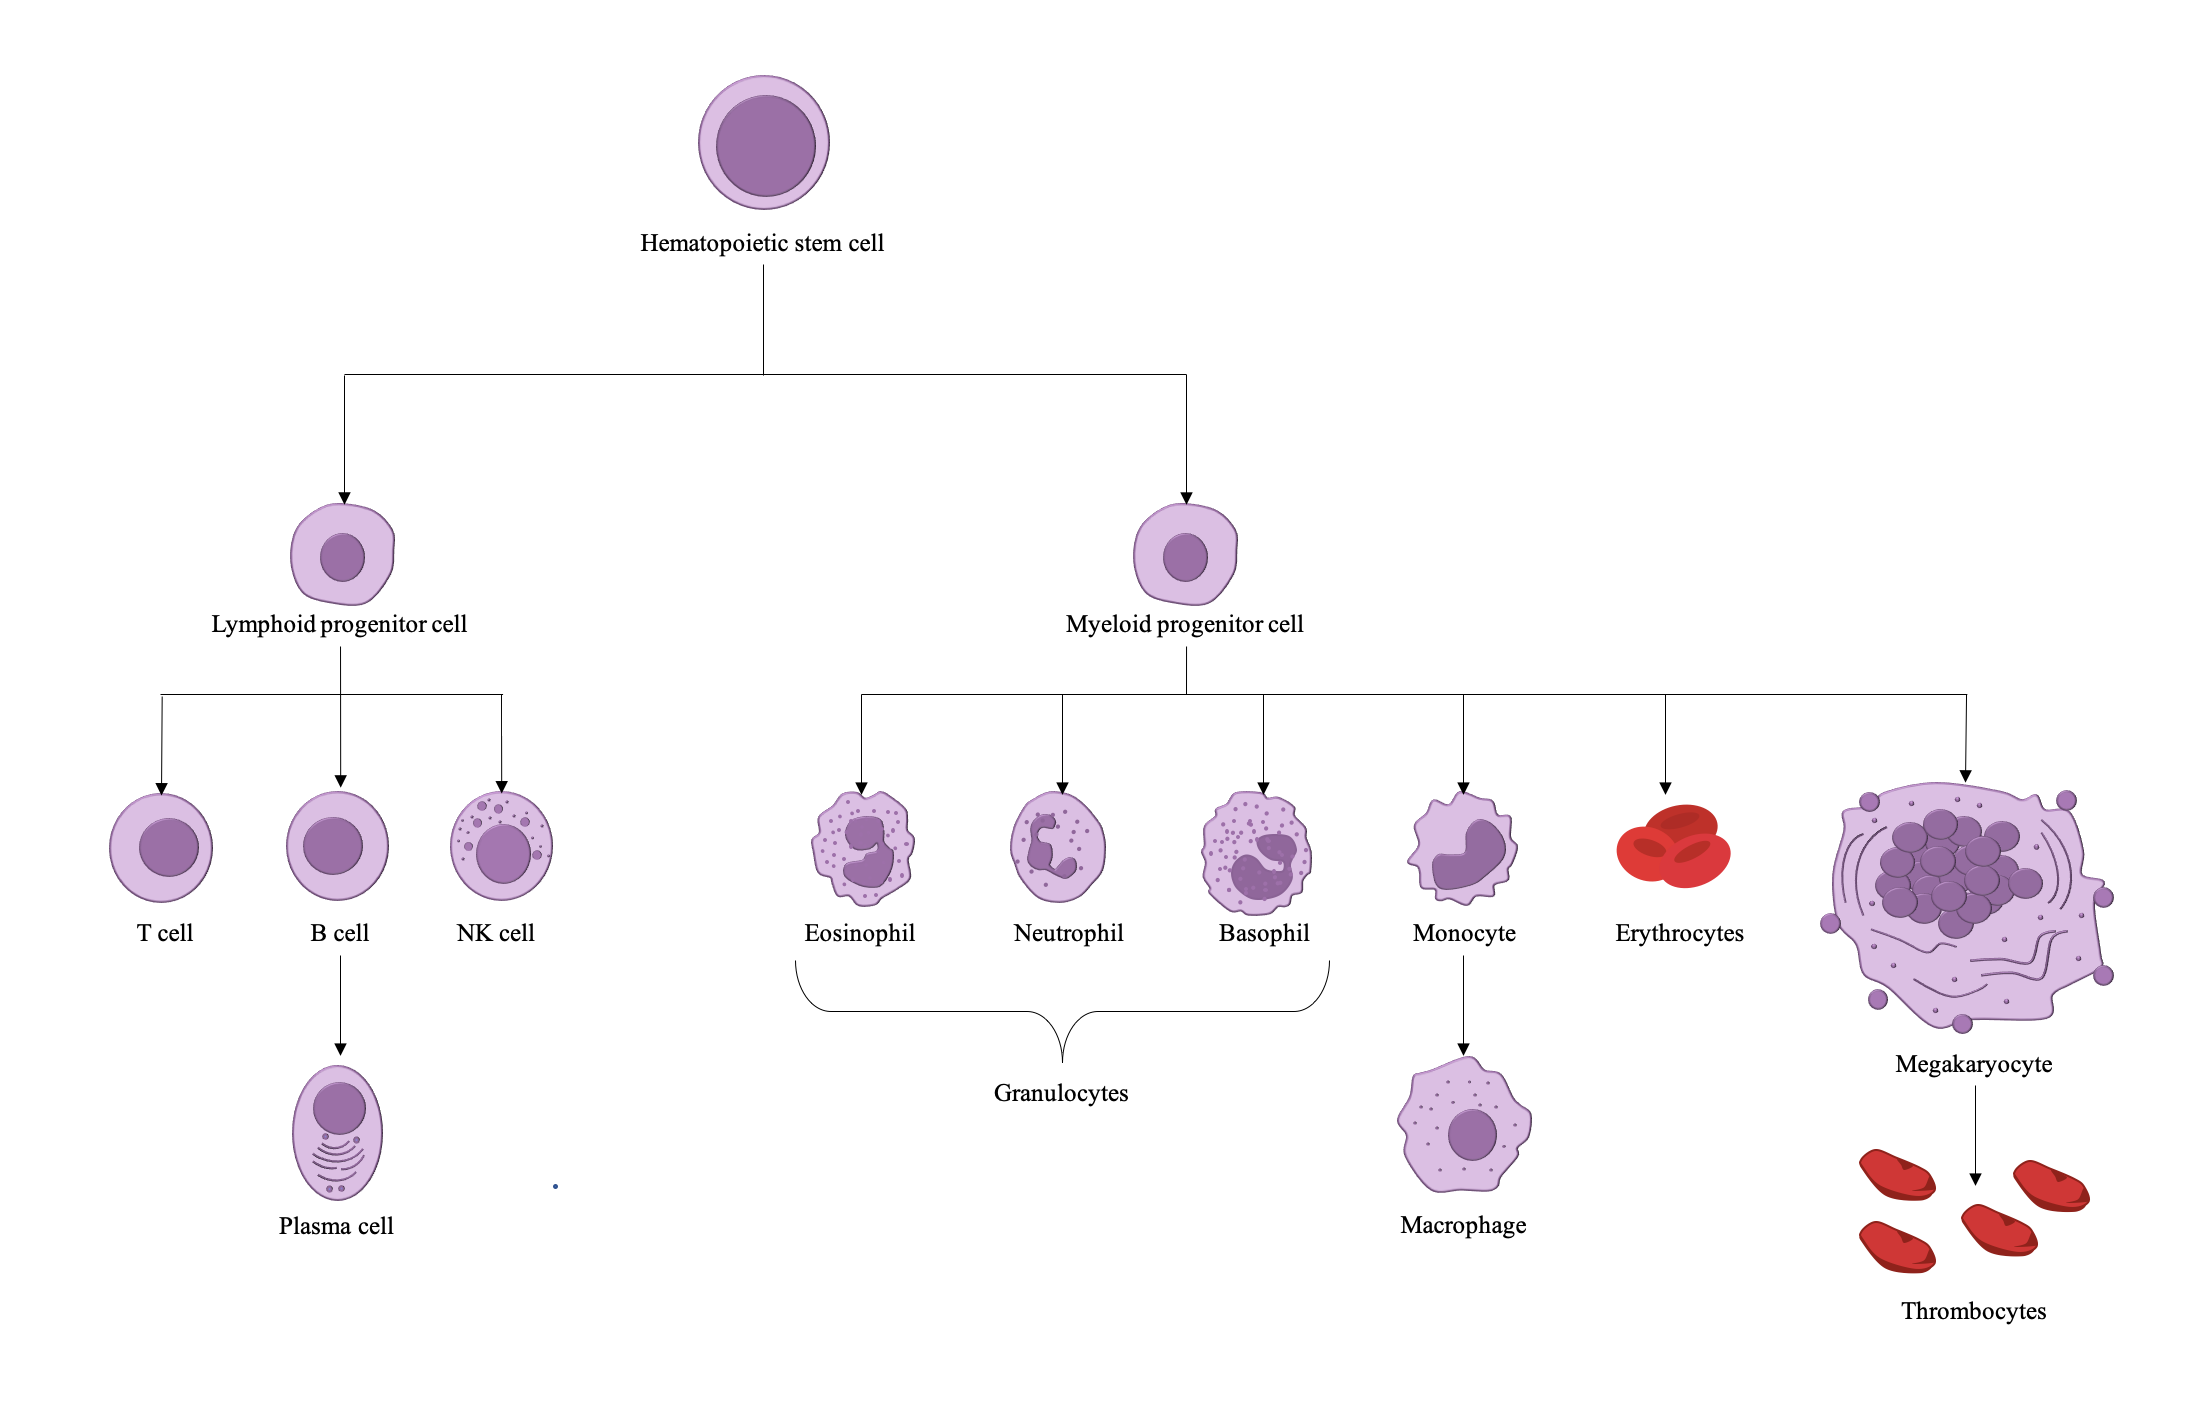
\includegraphics[width=\textwidth]{figures/Introduction/immune_cells.pdf}
\caption[Hematopoietic system cell differentiation]{Hematopoietic stem cell (HSC) differentiation.
Multipotent HSCs divide and either self-renew or commit to common myeloid or common lymphoid progenitor cells.
The committed progenitor cells then further commit to progressive restrictive progenitors, then finally differentiated cells such as B cells, T cells, macrophages and erythrocytes.
In adult mammals, all cells shown develop in the bone marrow, except for T cells, which develop in the thymus, and macrophages, which develop from blood monocytes.
Numerous dendritic cell phenotypes exist, they can be derived from lymphoid and myeloid progenitors, as well as monocytes.}
\label{fig:HSC_differentiation}\end{figure}
%%
Stem cells are precursor cells which can give rise to at least one type of differentiated (mature) cell, with the capability of indefinite self-renewal.
HSCs divide to either generate more HSCs (self-renewal) or committed progenitor cells.
HSCs are thought to go through stages of progressive restrictive commitments, until they eventually become fully differentiated blood cells such as NK cells, T cells and macrophages (Figure \ref{fig:HSC_differentiation}).
Firstly, HSCs lose self-renewal capacity, then commit to either a myeloid or lymphoid fate.
Myeloid progenitors give rise to monocytes, macrophages, granulocytes (neutrophils, eosinophils, basophils), mast cells, megakaryocytes and erythrocytes (red blood cells).
Lymphoid progenitors give rise to natural killer (NK) cells, T cells and B cells.
Both myeloid progenitors and lymphoid progenitors can produce dendritic cells (DCs)\cite{alberts2007molecularstem}.
Each stage of commitment correlates with changes in expression of specific genes and transcriptional regulators, for the given subset of blood cells\cite{seita2010hematopoietic}.

\subsection{The innate immune response}
The innate immune response, or `non-specific immunity', is the first defence a host has to prevent infection from invading pathogens\cite{alberts2007molecularimmune}.
Innate immunity is found in all species, from early multi-cellular organisms to humans\cite{hoffmann2013innate}.
Innate immunity comprises physical barriers, such as tight junctions in the skin and epithelial/mucous membranes, as well as defensive cell-coordinated responses.
Once foreign pathogens enter the host, numerous signalling cascades are initiated.
Host cells are able to recognise foreign microbials by characteristic features, known as pathogen-associated molecular patterns (PAMPs).
Once PAMPs are recognised by host pattern recognition receptors (PRRs), inflammatory responses are triggered and the invading pathogen is targeted for phagocytosis.
Phagocytic cells, for example neutrophils, monocytes and macrophages (Figure \ref{fig:HSC_differentiation}), non-specifically engulf foreign pathogens, and use a combination of toxic molecules, degradative enzymes and antimicrobial peptides to kill the invaders.
Additionally, various cytokines and inflammatory mediators are released.
NK cells directly kill host cells infected by a virus\cite{alberts2007molecularimmune} and an array of tumour cells\cite{hoffmann2013innate}.

In addition to its role preventing infection and eliminating invading pathogens, the innate immune response also stimulates the acquired immune response.
Dendritic cells act as a functional link between innate immunity and the adaptive immune response.
DCs become activated after they phagocytose microbes, they then cleave the microbial proteins, which bind to MHC proteins and together are transported to their cell surface.
The activated DCs then carry the peptide-MHC complexes to lymphoid organs, which in combination with DC-secreted cytokines and expression of co-stimulatory proteins and cell-cell adhesion molecules, activate T cells to initiate the adaptive immune response.
Innate immunity is a fast response (minutes to hours), whilst adaptive immunity takes longer (days to weeks)\cite{alberts2007molecularimmune}.

\subsection{The adaptive immune response}
During evolution, vertebrates have also developed adaptive immune responses, in addition to innate responses\cite{hoffmann2013innate}.
Adaptive immune responses are specific to the pathogen that induced the response.
Adaptive immunity is dependent on millions of B cells and T cells clones.
Each clone shares a unique cell-surface receptor that can bind to a specific pathogen antigen.
These receptors are antigen selective, they can distinguish between stereo isomers of the same molecule, and proteins differing by one single amino acid.
Two classes of adaptive immune responses exist: antibody responses, co-ordinated by B cells, and cell mediated immune responses, co-ordinated by T cells\cite{alberts2007molecularimmune}.
%The success of the adaptive immune system is dependent on the ability to respond to a diverse number of different antigenic stimuli and the long-term effectiveness of this response.
%
\subsubsection{T cells}
T cells are predominantly produced in the thymus (hence their name).
T cells are activated by fragments of partially proteolysed antigens displayed on the surface of antigen presenting cells (APCs), for example dendritic cells or macrophages.
T cells recognise these fragments with their cell-surface T cell receptors (TCRs)\@.
All effector T cells interact with other host cells in the body, therefore have a short range of effect\cite{alberts2007molecularimmune}.

There are three main classes of T cells: cytotoxic (T\textsubscript{C}) T cells, helper T (T\textsubscript{H}) cells and regulatory T (T\textsubscript{reg}) cells.
Effector cytotoxic T cells express CD8 co-receptors (CD8\textsuperscript{+} T cells) and act like NK cells by directly killing infected host cells, protecting against intracellular pathogens.
Effector helper and regulatory T cells express CD4 co-receptors (CD4\textsuperscript{+} T cells)\cite{luckheeram2012cd4}.
Helper T cells work by activating other host cells in the innate and adaptive immune system, for example, by activating B cells to secrete antibodies and undergo class switching, by helping activate macrophages to destroy intracellular pathogens, recruiting neutrophils and promoting pro-inflammatory cytokine production, and inducing naive cytotoxic T cells to become effector cells.
Helper T cells can be further divided into T\textsubscript{H}1, T\textsubscript{H}2, T\textsubscript{FH} and T\textsubscript{H}17 subclasses\cite{alberts2007molecularimmune,luckheeram2012cd4}.
Regulatory T cells have the opposite function to helper T cells.
T\textsubscript{reg}s prevent an excessive immune response that could be potentially harmful to the body.
The development, activation and function of other immune cell types is suppressed by T\textsubscript{reg}s by secreting suppressive cytokines such as TGF$\beta$ and interleukin (IL)-10, and inhibitory cell-surface proteins.
This means that the response to harmless ingested or inhaled antigens is limited\cite{alberts2007molecularimmune}.

%
\subsubsection{B cells}
B cells and plasma cells produce immunoglobulins (Igs).
Immunoglobulins (Ig) are typically large Y-shaped proteins.
The function of immunoglobulin molecules is to recognise and bind specific foreign antigens on pathogens.
Binding of immunoglobulins to antigens renders the virus or microbial toxin inactive as it blocks their ability to bind to host cells.
Additionally, Ig binding makes it easier for phagocytic cells to ingest the pathogen\cite{alberts2007molecularimmune}.
%%
%% Antibody figure
\begin{figure}[htb]
\centering\includegraphics[width=\textwidth]{figures/Introduction/immunoglobulins.pdf}
\caption[Immunoglobulins]{Immunoglobulin (Ig) diagram.
a) A bivalent immunoglobulin molecule (specifically IgG).
Igs are comprised of two identical heavy chains and two identical light chains.
Each chain has a constant region ($\kappa$ or $\lambda$ for light chains, and $\gamma$, $\epsilon$, $\delta$, $\alpha$ or $\mu$ for heavy chains), and a variable region.
Hypervariable regions are domains on heavy and light chains that come in direct contact with antigens.
These regions are frequently mutated to allow binding of diverse antigens.
The two heavy chains are covalently linked by disulfide bonds in their hinge regions.
Hinge regions offer flexibility which improves antibody-antigen binding efficiency.
Heavy and light chains are held together by a mixture of covalent disulfide bonds (red) and non-covalent bonds.
b) The five major classes of Igs in humans: IgG, IgE, IgD, IgA and IgM, in their main secretory (antibody) form.
IgE and IgM have no hinge regions and are composed of four heavy chain constant regions, not three.
IgA and IgM are shown in their dimer and pentamer polymer formations, however other polymer formations are also found in the body.}
\label{fig:immunoglobulins_diagram}\end{figure}
%%

Some Igs in circulation are found in polymer formations of multiple Ig units, such as dimers or pentamers.
A single Ig unit consists  of two identical heavy chains and two identical light chains (Figure \ref{fig:immunoglobulins_diagram}a).
Each heavy and light chain has a constant region and a variable region.
Heavy chains consist of one variable domain, and three or four constant domains.
Light chains consist of one variable domain and one constant domain.
Constant regions are found at the C-terminal end of Igs, and are a constant sequence for each given chain type.
Variable regions are found at the N-terminal end of Igs.
The variable regions of the heavy and light chain form the antigen-binding sites of Igs.
The amino acid sequence variation of variable domains confer diversity for antigen-binding.
Both chains also contain hypervariable regions, which come in direct contact with antigens.
These domains are frequently mutated to allow for even more diversity of antigen binding\cite{schroeder2010structure}.

Humans produce five main isotypes of immunoglobulin: IgM, IgD, IgG, IgA and IgE (named after the greek letter of their respective heavy chain; Figure \ref{fig:immunoglobulins_diagram}b).
IgG can be divided into 4 subclasses, IgG1, IgG2, IgG3, and IgG4, and IgA can be divided into IgA1 and IgA2\cite{schroeder2010structure}.
Igs can either be membrane-bound (mIgs) on the cell-surface or secreted (sIgs, also called antibodies).
Naive B cells only produce mIgs-- they do not secrete antibodies.
IgM molecules are the first immunoglobulins produced by newly formed B cells.
Membrane IgMs (mIgMs) associate with two signalling proteins Ig-$\alpha$ and Ig-$\beta$; these complexes are known as B-cell antigen receptors (BCRs)\cite{friess2018structural, dylke2007role}.

% During B cell development in the bone marrow, each B cell's antigen
Each B cell's individual Ig antigen-binding site is determined by a process called V(D)J recombination, whereby separate Ig gene segments are joined together.
Separate loci, on three separate chromosomes code for $\kappa$ light chain (chromosome 2), $\lambda$ light chain (chromosome 22) and the heavy chains (chromosome 14).
Each light chain locus consists of one or more coding sequence for constant (C) regions, and a set of variable (V) and joining (J) sequences.
The heavy chain locus contains these elements plus an added diversity (D) gene segment.
These gene segments are rearranged and brought together by site-specific recombination, aided by V(D)J recombinase enzyme.
The RNA that codes for the whole Ig polypetide chain is produced by co-transcribing the constant regions and variable regions together.
From all the potential combinations of V, D and J gene segments, in theory, over 1.5 million different antigen-binding sites could be made.
Diversity of antigen-binding sites is further increased by junctional diversification, whereby variable numbers of nucleotides are lost or randomly inserted at joining sites.
This can increase diversity of variable coding sequences by $10^8$ fold.
However, this process can also shift the reading frame to produce non-functional genes.
B cells that produce non-functioning Igs subsequently die in the bone marrow.
Additionally, B cells that produce BCRs that bind too strongly to self-antigens in the BM undergo another round of V(D)J recombination to alter specificity; if this fails again then B cells die by apoptosis.
Once a B cell can produce functional Igs, the V(D)J recombination process is switched off, and it only makes Igs with the same antigen specificity\cite{alberts2007molecularimmune}.

\subsection{B cell maturation}
Most B cells die in the bone marrow soon after developing, however some will develop in the bone marrow, where initial stages of maturation occur and then migrate to secondary lymphoid organs, such as the spleen.
Within secondary lymphoid organs, numerous critical decisions on B cell fate are made, involving complex transcriptional networks, cell interactions, gene rearrangements, and mutations\cite{roth2014tracking, jourdan2011characterization}.
As B cells develop and leave the bone marrow to populate peripheral lymphoid tissues, they undergo alternative mRNA splicing and start to express IgD BCRs in addition to IgM; they are henceforth known as mature naive B cells.
IgM and IgD BCRs on a single mature naive B cell all contain identical antigen-binding sites.
To fully differentiate, B cells require antigen stimulation.
Upon antigen stimulation, mature naive B cells are activated to differentiate into either Ig-secreting effector B cells (plasma cells) or memory B cells.
Terminally differentiated plasma cells are the final effectors of the B cell lineage.
Plasma cell differentiation involves the loss of expression of many genes, such as \textit{CD19}, \textit{CD20} and increased expression of plasma cell markers, such as \textit{CD138} and \textit{CD38}.
Plasma cells have an extensive rough endoplasmic reticulum (ER), and have numerous genes involved in antibody secretion upregulated, including \textit{XBP1} and \textit{CHOP}, to enable the production of copious amounts of antibody\cite{shapiro2004plasma}.
Antibodies recognise and bind to the specific foreign antigen on the pathogen which stimulated their production.
Binding of antibodies to antigens renders the virus or microbial toxin inactive as it blocks their ability to bind to host cells.
Additionally, antibody binding makes it easier for phagocytic cells to ingest the pathogen\cite{alberts2007molecularimmune}.

Initially, effector B cells only secrete primary Igs (IgM and IgD) that have low binding affinity for antigens.
However, further antigenic-stimulation, helper T cell activation, various cytokine secretions and activation-induced-deaminase (AID) enzyme activity, leads to processes which increase binding affinity of antibodies (affinity maturation) and diversify Ig isotype production (class switching).
The main stages of B cell maturation can be seen in Figure \ref{fig:b_cell_mat}.

%% B cell maturation figure
\begin{figure}[htb]
\centering\includegraphics[width=\textwidth]{figures/Introduction/b_cell_maturation.pdf}
\caption[B cell maturation]{A simplified diagram of B cell maturation.
Once hematopoietic stem cells (HSC) commit to the B cell lineage, the cells undergo a number of changes in the bone marrow and secondary lymphoid tissues until they eventually commit to either becoming antibody-secreting plasma cells or memory B cells.
}
\label{fig:b_cell_mat}\end{figure}
%%

\subsubsection{Affinity maturation}
Affinity maturation occurs through a process known as somatic hypermutation, whereby activated B cells form germinal centres and their variable regions mutate at a rate approximately a million times greater than spontaneous mutations.
The enzyme AID is required for this process.
Not many of the Igs that undergo hypermutation will have a stronger affinity for the antigen present.
However, B cells produce BCRs and antibodies, both of which contain the same antigen-binding site.
The B cells with a higher affinity antigen-binding site for the given antigen, will be preferentially stimulated at their BCRs.
This in turn means that clones with increased affinity will preferentially proliferate and survive over other B cells with lesser affinity (similar to how evolution and natural selection works in population genetics).
Most other B cells in the germinal centre will undergo apoptosis and die.
After numerous repeated cycles of mutation and selection, the remaining effector B cell clones will have improved Ig affinity 10--5000 fold for the antigen during the course of the immune response\cite{mishra2018insights}.

\subsubsection{Class switching}
Class switching often occurs after somatic hypermutation has taken place, however they are independent processes, and B cells can class-switch without having already undergone somatic hypermutation\cite{mak2014b}.
Various cytokines produced by activated T helper cells, such as IFN$\gamma$ produced by T\textsubscript{H}1 cells, IL-4 and IL-5 produced by T\textsubscript{H}2 cells and IL-21 produced by T\textsubscript{FH}, can promote B cell class/isotype switching.
Class switching allows effector B cells to produce the secondary class of Igs: IgG, IgA and IgE\@.
Class switching is dependent on the mechanism `switch recombination', where the constant heavy chain region undergoes a number of DNA cutting/rejoining events that bring any of the secondary Igs constant heavy chain exons adjacent to heavy VDJ exon\cite{mak2014b}.
The mechanism is not yet fully understood, however AID is necessary to facilitate class switching.
Daughter cells from the same effector B cell will then be able to produce different isotypes of Igs, but all retaining their original specific antigen-binding site.
In the early stages of an immune response, IgM is the main circulating antibody.
After a lag period, IgG becomes the main circulating antibody in the blood\cite{alberts2007molecularimmune}.

The Ig isotypes have distinct immune functionality and tissue distribution.
For example, a portion of IgG molecules can bind to macrophages and neutrophils, aiding in phagocytosis of microorganisms, it is also the only Ig that can cross the placenta; IgE molecules can bind to mast cells and basophils, and play a large role in allergic reactions and parasitic infections; IgA molecules are the main antibody in bodily secretions\cite{alberts2007molecularimmune}.
By each Ig class retaining the same antigen-binding site, this means that antigen-specificity can be distributed amongst the various isotypes.
Therefore, a pathogen can be fought using an array of each isotype's biological properties\cite{xu2012immunoglobulin}.

% Secreted bind to phagocytes with tail
%Prior to antigenic-stimulation, V(D)J recombination increases the diversity of a human's primary Ig repertoire, and allows for production of an almost limitless pool of antibodies.
%Once a B cell is activated, class switching increases the diversity of Ig isotypes available to a cell and therefore the capacity of immune functionality, and affinity maturation/somatic hypermutation greatly increases the affinity of antigen-binding sites for the given antigen.

\subsubsection{Immunological memory}
Following antigenic-stimulation, B cells proliferate and differentiate into either antibody-secreting plasma cells or memory B cells.
Memory B cells are long-lived, quiescent cells that possess the ability to `remember' past pathogens and respond quickly to the antigen\cite{palm2019remembrance}.
Memory B cells express BCRs of various Ig isotypes.
Plasma cells appear to consist of two distinct categories: short-lived plasma cells, which have life-spans of several months and are located in extrafollicular locales such as in medullary chords of lymph nodes or the red pulp of the spleen, and long-lived plasma cells (LLPCs), which have a much longer life-span, ranging from months to decades\cite{bortnick2013and, andraud2012living}.
LLPCs are mainly found in the bone marrow\cite{bortnick2013and, andraud2012living}.
At the end of a primary immune response (first exposure to an antigen), the majority of antigen-specific B cell clones undergo apoptosis, leaving memory cells and LLPCs as the only remaining cells from the B cell lineage.
Upon second exposure to an antigen, these cell types speed up the secondary immune response and reduce the lag period seen in the primary immune response.
Existing memory B cells, which already possess high-affinity receptors for the given antigen, are expanded for immediate differentiation into short-lived plasma cells that can secrete high affinity antibodies.
Human memory B cells can be split up into three main categories: IgM\textsuperscript{+} only, IgM\textsuperscript{+}IgD\textsuperscript{+}, and class switched IgG\textsuperscript{+} and IgA\textsuperscript{+}\cite{palm2019remembrance}.
IgG\textsuperscript{+} memory B cells are more likely to differentiate into plasma cells following re-infection.
Immunological memory is the basis for the success of vaccinations, where previous exposure to a weakened/dead microorganism or its protein/toxin stimulates an immune response and `readies' the body for if it encounters the full disease.
%A secondary immune response to an antigen (either due to vaccination or previous infection), will often have a shorter lag period than a primary immune response, as there are pre-existing B and/or T cells with specificity for the antigen.
%There is evidence that LLPCs as well as memory B cells contribute to immunological memory and fast and effective responses to repeat antigen contact\cite{ionescu2019memory}.
%%%%%%

%1
\section{Multiple myeloma}\label{sec:MM}
%2
\subsection{Multiple myeloma cells}
Multiple myeloma (MM) is a malignancy of terminally differentiated plasma cells.
It is characterised by aberrant proliferation of clonal, long-lived plasma cells in the bone marrow\cite{anderson2011pathogenesis}.
The large accumulation of MM cells displace healthy cells in the bone marrow.
Under normal conditions, plasma cells produce antibodies that fight infection as part of the adaptive immune system.
However malignant plasma cells (MM cells) produce large amounts of abnormal antibodies that are unable to fight infection, coined `paraproteins' or `M proteins' (Figure \ref{fig:m_spike}).
%
%% M spike
\begin{figure}[htb]
\centering
\includegraphics[width=\textwidth]{figures/Introduction/M_spike.pdf}
\caption[SPEP M spike]{Diagram of serum protein electrophoresis (SPEP) for a healthy individual and for a multiple myeloma (MM) patient.
Based on proteins' electrical charge, size and shape, SPEP separates proteins in blood.
A large peak is recorded for albumin (the most abundant protein in blood), followed by lower levels of the other proteins, grouped into $\alpha1$, $\alpha2$,$\beta$ and $\gamma$ regions.
Antibodies are located in the $\gamma$ region.
The large quantities of a single type of antibody (M protein) produced by MM cells cause a distinct, narrow `M spike' in the $\gamma$ region.}
\label{fig:m_spike}
\end{figure}
%%
Only one type of Ig is overproduced by a MM patient.
The type of Ig overproduced varies from patient to patient.
Paraproteins can either be whole Igs or just the light chain ($\kappa$ or $\lambda$) part of an Ig, or more rarely, just the heavy chain (Figure \ref{fig:immunoglobulins_diagram}a).
A patient's myeloma type is named after the abnormal Ig isotype they are making.
IgG is the most common type, followed by IgA and light-chain-only myeloma.
IgM, IgD and IgE are very rare myeloma types\cite{cancerresearchuktypes}.
Increased IgM can also be seen in other B cell malignancies such as Waldenstrom's macroglobulinemia, which is a rare proliferative disease of B lymphocytes.

Malignant MM cells vary from healthy plasma cells considerably.
The transformation from healthy plasma cell to MM cell is a complex multi-step process, involving numerous genomic, epigenomic, transcriptomic, proteomic and metabolic changes\cite{de2002comparison, caprio2020epigenetic, chanukuppa2021proteomic, el2018metabolic}.
Examples of such genomic changes include a rearrangement of the 14q32 locus (where the Ig heavy chain gene is located)\cite{nishida1997ig} in approximately 60\% of patients, as well as rearrangements in \textit{MYC}, \textit{CCND1}, \textit{FGFR3} and \textit{CCND3}\cite{de2002comparison}.
Fluorescence in situ hybridization (FISH) testing is often performed on upon MM diagnosis and at time of relapse, to detect certain genetic alterations and aid in risk stratification of patients\cite{swerdlow2008classification}.
Deletions of chromosome 13 and mutations in \textit{NRAS} and \textit{KRAS} are also frequently seen in MM\@.
Gene expression changes in MM cells include loss of \textit{CD19} expression and aberrant \textit{CD56} expression.
DNA methylation and histone modifications have also been indicated as crucial regulators of MM pathogenesis.

\subsection{MM microenvironment}
MM cells typically grow within the bone marrow (BM).
This is often referred to as their BM niche or BM microenvironment.
The surrounding microenvironment plays a large role in supporting the progression of MM\@.
The BM microenvironment is comprised of a cellular compartment (immune cells, endothelial cells, osteoblasts, osteoclasts and stromal cells) and a non-cellular compartment (the extracellular matrix (ECM), cytokines, chemokines and growth factors)\cite{manier2012bone, kawano2015targeting}.
MM cells interact with their surrounding environment.
These interactions influence the migration, differentiation, survival, proliferation, and response to therapies of MM cells.

%2
\subsection{Epidemiology}
MM accounts for 1-2\% of all cancers and has the second highest incidence of hematological malignancies, after non-Hodgkin's lymphoma\cite{international2003criteria}.
MM is rare in individuals under the age of 40, with a median age of 70 at time of diagnosis\cite{tsang2019multiple, palumbo2011multiple}.
MM is more prevalent in males than females and is around twice as common in black populations than in Caucasian or Asian populations\cite{nhsmyeloma}.
The average incidence rate is approximately 1-6 cases per 100,000 individuals\cite{tsang2019multiple, palumbo2011multiple, teras20162016}, with the highest age-standardised incidence rates in the regions of Australasia, North America, and Western Europe\cite{cowan2018global}.
Five-year survival rate of MM patients is approximately 49\%, whilst approximately a third of MM patients survive ten years or greater\cite{cancerresearchuk, siegel2016cancer}.
%While there have been many successful medicines developed for myeloma, they all suffer from the development of drug resistance.

%2
\subsection{Presentation of precursor states}
%3
All cases of MM are preceded by asymptomatic precursor states, monoclonal gammopathy of unknown significance (MGUS) and smouldering multiple myeloma (SMM).
However, only some patients with SMM or MGUS progress to active MM\@.

MGUS is a pre-malignant condition where patients have the presence of monoclonal immunoglobulins in their blood or urine, $<$10\% clonal plasma cells in their bone marrow, but lack any myeloma-related end-organ damage\cite{van2018mgus}.
Patients with SMM have between 10\% and 60\% clonal plasma cells in their bone marrow, serum monoclonal immunoglobulin of $\ge$3 g/dL, and like MGUS, have no signs of end-organ damage\cite{rajkumar2015smoldering}.
Progression risk of MGUS into symptomatic MM is about 1\% per year, whilst progression risk of SMM to MM is higher, at around 10\% per year for the first 5 years, after which it decreases\cite{korde2011monoclonal, kyle2007clinical}.
%

%3
\subsection{Presentation of active MM}
There are multiple classifications of active MM\@.
The International Myeloma Working Group's definition\cite{rajkumar2014international} is as follows:
greater than 10\% clonal plasma cells located in the bone marrow and one or more myeloma-defining event or biomarker of malignancy.
Myeloma defining events consist of evidence of end-organ damage that can be attributed to the surplus of M protein and clonal plasma cells, namely the CRAB features:
%
% List of myeloma events (CRAB)
\begin{itemize}
  \item Hypercalcemia (C)
    \begin{itemize}
        \item Increased serum calcium
        \item Symptoms include: excessive thirst, nausea, constipation, tiredness, loss of appetite, excessive urination and confusion
    \end{itemize}
  \item Renal dysfunction (R)
    \begin{itemize}
        \item Increased serum creatinine levels
        \item Symptoms include: nausea, loss of appetite and weight loss, dehydration, tiredness and lack of energy, swollen feet and hands
    \end{itemize}
  \item Anaemia (A)
    \begin{itemize}
        \item Anaemia of unknown cause
        \item Decreased hemoglobin levels
        \item Symptoms include: breathlessness and tiredness
    \end{itemize}
    \item Bone lesions (B)
      \begin{itemize}
        \item Unexplained and persistent bone pain (often in the back, shoulders, hips or ribs)
        \item Osteolytic lesions found using skeletal radiography, computerized tomography (CT) or positron emission tomography (PET)-CT scans
        \item Symptoms include: pain, breaks/fractures, and spinal problems.
      \end{itemize}
\end{itemize}
% End of list
%

\noindent
MM patients are also more prone to infections, and often take longer to recover from illness.
This is because MM patients do not have enough healthy white blood cells to fight pathogens effectively.
Biomarkers of malignancy include greater than or equal to 60\% clonal plasma cells in the BM, an involved-to-uninvolved serum free light chain ratio greater than or equal to 100, and more than one focal lesion on an MRI study\cite{rajkumar2014international}.

It is currently unclear what causes the malignant transformation between precursor states and active MM\@.
Certain factors have been identified as risk factors, including point mutations in genes such as \textit{NRAS}, \textit{KRAS} and \textit{MYC}; chromosomal copy number variations, for example deletion of chromosome 13; a large array of up-regulated transcription factors, such as \textit{MYC}; and numerous changes to the immune system\cite{korde2011monoclonal, mccachren2021co}.
The shift from MGUS and SMM to active MM is extremely complex, multiple stages of transformations are undergone and the genetic landscape changes considerably over the course of the disease.

\subsection{Treatment of MM}\label{subsec:mm_treatment}
Multiple myeloma may be an incurable disease, however it is treatable.
In fact, in the last decade median survival time for newly diagnosed MM patients has almost doubled\cite{kazandjian2016look}.
Novel therapeutic advances have contributed to this improvement (Table \ref{tab:treatment_history}).
Myeloma is usually treated with a combination of drugs, often comprising a corticosteriod, a proteasome inhibitor, and an immunomodulatory drug (IMiD).
A common regimen, approved in the USA, European Union and UK for untreated myeloma is the triplet VRd regimen.
This consists of the proteasome inhibitor bortezomib (brand name Velcade), the IMiD lenalidomide (brand name Revlimid), and the corticosteroid dexamethasone.
More commonly in the UK (via the NHS), bortezomib (Velcade), thalidomide and dexamethasone (known as VTd) is used as an initial treatment for MM\@.
Recently, the regimen DVTd has been introduced in the UK, which is the above triplet combined with the anti-CD38 monoclonal antibody daratumumab (Darzalex).
DVTd has been shown to improve progression-free survival and response rates in MM patients compared to VTd.
Additionally, any MM patients who are eligible (based on frailty, age, organ function and comorbidities) receive high-dose chemotherapy followed by autologous stem cell transplantation (HDT-ASCT) as standard treatment.

% Timeline of treatment options
%% Table for treatment timeline


\begin{table}[h]
\centering
\begin{tabular}{|p{1cm}|p{3cm}|p{8cm}|p{1.3cm}|}
\hline
\textbf{Year} & \textbf{Treatment} & \textbf{Usage} & \textbf{Ref} \\ \hline
1958 & Melphalan & The alkylating agent melphalan was first used in plasma cell myeloma in 1958. & \cite{blokhin1958clinical} \\ \hline
1960s & Corticosteroids & Placebo-controlled double-blind trial of prednisone in multiple myeloma. Combinations of prednisone and melphalan showed an increased survival over melphalan alone. Dexamethasone and prednisone have become a cornerstone in the treatment of multiple myeloma. & \cite{mass1962comparison, alexanian1969treatment} \\ \hline
1980s & Stem-cell transplantations & Numerous successful allogenic and autologous bone marrow transplantations in patients with multiple myeloma &  \cite{mcelwain1983high, osserman1982identical, fefer1986identical, gahrton1987bone}  \\ \hline
2003 & Proteasome inhibitors & Bortezomib, a first-in-class proteasome inhibitor, was first approved by the FDA for use in relapsed and refractory multiple myeloma. In 2008 it was approved for patients with no prior treatment. Carfilzomib was approved in 2012 for advanced MM and later in 2015 for treatment of relapsed MM. The oral proteasome inhibitor, ixazomib, was approved as a combination treatment with lenalidomide and dexamethasone in 2016 for people who have received at least one previous treatment. & \cite{kane2003velcade,richardson2003phase,katsnelson2012next} \\ \hline
2006 & IMiDs & The antitumour activity of thalidomide was demonstrated in 1999, this led to the development of lenalidomide, the first approved immunomodulatory imide drug (IMiD) for use in multiple myeloma. Currently, thalidomide, lenalidomide and pomalidomide are approved for use in multiple myeloma & \cite{singhal1999antitumor,label47revlimid,san2013pomalidomide} \\ \hline
2015 & Monoclonal antibodies & In 2015, daratumumab, an anti-CD38 monoclonal antibody and elotuzumab, an anti-SLAMF7 monoclonal antibody, were approved for MM treatment. & \cite{lokhorst2015targeting,lonial2015elotuzumab} \\ \hline
\end{tabular}
\caption[Timeline of treatment options for multiple myeloma]{Timeline of treatment options for multiple myeloma. Listed by first usage or FDA approval for MM.}
\label{tab:treatment_history}
\end{table}

% https://www.ncbi.nlm.nih.gov/pmc/articles/PMC5282737/
% https://www.ncbi.nlm.nih.gov/pmc/articles/PMC2265446/
% Panobinostat	HDACi
% Liposomal doxorubicin	DNA inter-calator



\subsubsection{Proteasome inhibitors}
Proteasome inhibitors have contributed greatly to the improved prognosis of MM since their introduction into treatment regimes.
The first-in-class proteasome inhibitor bortezomib (Velcade; BTZ) was approved by the FDA in 2003 as a single-agent for injection of relapsed MM\cite{kane2003velcade}.
Since then it has been approved for use in combination therapies.
Bortezomib in combination with melphalan-prednisone proved to be superior to the previous standard of care for patients ineligible for HDT-ASCT of melphalan-prednisone alone, increasing progression free survival\cite{san2008bortezomib}.
The combination of bortezomib, dexamethasone and thalidomide  was also shown to be superior to previous standard of care for patients prior to ASCT\cite{moreau2012proteasome}.
In 2010, bortezomib was approved as a frontline therapy for treatment-naive MM patients.
Since then, two more proteasome inhibitors have been approved, carfilzomib (CFZ) and ixazomib.
Carfilzomib is structurally and mechanistically different to bortezomib and shows activity on bortezomib resistant primary MM cells\cite{moreau2012proteasome}; it is approved for relapsed or refractory MM\@.
Additionally, CFZ and BTZ have different side effect profiles.
BTZ treatment displays side effects such as peripheral neuropathy (PNP).
PNP has been reported in up to 30\% of MM patients treated with BTZ-based regimens\cite{mushtaq2018efficacy}.
CFZ treatment has lower rates of PNP, however is associated with significant incidence of cardiovascular adverse events (heart failure, hypertension, ischemia, and arrhythmias)\cite{waxman2018carfilzomib}.
In relapsed MM patients, treatment choice often depends on prior therapy, recorded comorbidities and side effect profiles of the patient\@.

\subsubsection{The ubiquitin-proteasome system}
Proteasome inhibitors work by blocking the action of the proteasome in the cell.
Misfolded proteins can be harmful to a cell, so the combined activity of molecular chaperones, which aid in protein folding, and the ubiquitin-proteasome system (UPS), which acts to digest misfolded proteins, is needed to prevent aberrant protein aggregation.
Unneeded, misfolded or damaged proteins are tagged with lysine-48-linked poly-ubiquitin chains, marking them for degradation by the proteasome (Figure \ref{fig:26s_proteasome_structure}).
The proteasome is described as a complex `protein destruction machine'.
The proteasome consists of a 20S core particle, a central hollow cylinder, and 19S regulatory caps associated with each end of the cylinder.
The 19S regulatory caps perform substrate recognition, deubiquitination, unfolding and threading of the protein substrate into the 20S core.
The core is made up of four stacked heptameric ring structures.
The outer rings are responsible for docking to the 19S cap and for acting as a gate to the inner rings. The inner rings consist of seven $\beta$ subunits, containing inward-facing protease active sites for degrading proteins\cite{kleiger2014perilous, alberts2007molecular} (Figures \ref{fig:26s_proteasome_structure} and  \ref{fig:proteasome_beta_subunits}).

 % Proteasome structure diagram
\begin{figure}[ht]
%1
\begin{subfigure}[t]{0.5\textwidth}
    \includegraphics[width=\textwidth]{figures/Introduction/26s_proteasome_serif.jpg}
    \caption{26S proteasome}
    \label{fig:26s_proteasome_structure}
\end{subfigure}
%\medskip
\begin{subfigure}[t]{0.5\textwidth}
    \includegraphics[width=\textwidth]{figures/Introduction/20s_core_beta_subunits_serif.jpg}
    \caption{$\beta$-subunits of an inner ring of the 20S core particle }
    \label{fig:proteasome_beta_subunits}
\end{subfigure}
    \caption[Structure of the proteasome]{Structure of the proteasome.
    a) The structure of the 26S proteasome, comprised of the 19S regulatory caps and 20S core particle.
    A misfolded protein tagged with a poly-ubiquitin chain is recognised by the 19s regulatory cap, which cleaves the ubiquitins from the protein and threads the protein through to the core, where it is degraded into small peptides.
    The 20S core particle is made up of two outer rings of $\alpha$-subunits and two inner rings of $\beta$-subunits.
    b) The $\beta$-subunit arrangement of an inner ring of the 20s particle.
    $\beta1$ (caspase-like), $\beta2$ (trypsin-like) and $\beta5$ (chymotrypsin-like) are the proteolytically active subunits.
    Proteasome inhibitors are designed to primarily inhibit $\beta5$ subunits.}
\label{fig:proteasome_and_beta}
\end{figure}

\subsubsection{PI mechanism of action}
Of the seven proteasome $\beta$ subunits, only $\beta1$, $\beta3$ and $\beta5$ are proteolytically active (Figure \ref{fig:proteasome_beta_subunits}).
PIs are designed to target $\beta5$ as it has been shown as the rate limiting protease for proteasomal protein turnover\cite{besse2019proteasome}.
Bortezomib reversibly co-inhibits $\beta5$ and $\beta1$ subunits, whilst carfilzomib irreversibly binds to $\beta5$, with greater selectivity than bortezomib, and at higher doses binds to $\beta2$ as well\cite{besse2019proteasome}.

The precise downstream effects of $\beta$ subunit proteasome inhibition are not fully understood, however the unfolded protein response (UPR), NF-$\kappa$B signalling, JNK signalling, apoptotic factors and p53 are thought to be involved in the anti-MM effects\cite{kubiczkova2014proteasome}.
Specifically, the action of the UPR has been demonstrated as an important mechanism in the anti-MM effect of PIs.
MM cells secrete large amounts of monoclonal protein, leading to the rapid accumulation of  misfolded proteins within the endoplasmic-reticulum (ER) lumen.
This results in heightened ER stress, which is compensated by the UPR by reducing global protein translation and up-regulating UPS machinery\cite{wallington2018resistance}.
Therefore, by inhibiting the proteasome, fewer ubiquitin-tagged proteins are degraded and more misfolded proteins accumulate in the ER lumen.
ER stress is then further increased, causing the UPR to switch from a homeostatic, pro-survival system to a pro-apoptotic pathway\cite{kubiczkova2014proteasome, wallington2018resistance}.

Another important mechanism for PI activity is the attenuation of NF-$\kappa$B signalling. I$\kappa$B$\alpha$, a specific endogenous inhibitor of the transcription factor NF$\kappa$B, is a protein degraded by the proteasome.
Inhibition of the proteasome increases levels of I$\kappa$B$\alpha$, thereby abolishing NF$\kappa$B signalling.
NF$\kappa$B is a key transcription factor in many cancers, contributing to overall tumour growth and chemoresistance.
NF$\kappa$B has been shown to promote tumour cell proliferation, anti-apoptotic and angiogenic factors\cite{kale2012molecular}.

\subsection{Drug resistance in MM}
Although the standard therapeutics are effective at killing MM cells initially, long-term treatment inevitably results in a drug-resistant relapse.
Drug resistance is one of the biggest barriers in the treatment of MM, as in many other cancers.
Patients follow a pattern of peaks and troughs of treatment cycles, remission and relapse, until all therapies have little effect (Figure \ref{fig:treatment_cycles}).
%% Treatment cycles
\begin{figure}[htb]
\centering
\includegraphics[width=\textwidth]{figures/Introduction/treatment_cycles.pdf}
\caption[MM treatment cycles]{MM treatment cycles and disease progression over time.
All MM patients begin with precursor states monoclonal gammopathy of unknown significance (MGUS) and/or smouldering multiple myeloma (SMM) prior to a malignant transformation to symptomatic/active MM\@.
Patients undergo cycles of treatment, remission and relapse until eventually becoming relapsed and refractory (RRMM) and no longer responsive to treatment.
}
\label{fig:treatment_cycles}
\end{figure}
%%
\subsubsection{Minimal residual disease}
Minimal residual disease (MRD) is when a small number of cancer cells remain in the body after treatment.
These surviving cells are often undetectable and cause no symptoms, but they have the potential to proliferate and cause patients to relapse.
MRD status after treatment is used as a prognostic factor and a marker of therapeutic success.
Persistent MRD after a treatment cycle indicates that many MM cells were not killed and the patient is expected to relapse in the near future\cite{ding2021minimal}.
Clinical MRD negativity is defined as no cancer cells being detected in the background of at least $10^5$ normal cells by multi-parameteric flow cytometry (MFC) or next-generation sequencing (NGS) technology in MM patients who have achieved complete remission (CR)\cite{kumar2016international}.
Many studies have shown MRD negativity is positively associated with prolonged progression-free survival (PFS) and overall-survival (OS) in MM\cite{paiva2008multiparameter, martinez2014prognostic, munshi2020large}.


\subsubsection{Clonal evolution}
MM was originally thought to follow a linear pattern of evolution over time, however MM actually displays clonal evolution and intra-clonal heterogeneity, similar to `Darwinian' natural selection: individual clones compete for the same microenvironmental `niche' and limited resources, with anti-MM therapies acting as environmental selective pressure.
Three seminal papers from 2012 elucidated the clonal element of MM disease progression using time-course analyses of primary MM samples\cite{egan2012whole, keats2012clonal, walker2012intraclonal}.
These studies revealed substantial heterogeneity within tumour clones from the same patient (intra-patient heterogeneity).
Egan et al. (2012) collected DNA from a single MM patient over a five-year period, covering their initial diagnosis, first relapse, second relapse, and end-stage secondary plasma cell leukemia, and performed whole genome sequencing (WGS) on the samples\cite{egan2012whole}.
The group observed genomic sequence variants that were only detectable at alternating time points, suggesting the `waxing and waning' of different independent clones over time and treatment-courses, which rose and fell in dominance\cite{egan2012whole}.
Walker et al. (2012) further corroborated this finding and demonstrated intra-patient heterogeneity by identifying clonal and subclonal RAS mutations using whole exome sequencing (WES); this was also confirmed at the single-cell level\cite{walker2012intraclonal}\@.
It has since been shown that intra-patient heterogeneity is present at premalignant phases of MM (MGUS and SMM)\@.
On average, three to six major subclones are uniformly present at each stage of MM\cite{furukawa2020molecular}, although, this still might be a conservative estimate.
MM bone marrow aspirates are taken from a single site, usually the back of the hip bone.
Spatial genomic heterogeneity within MM, means there are probably far greater than six subclones present in a MM patient at one time, distributed across the whole body\cite{rasche2017spatial}.

Keats et al. (2012) described three distinct patterns for clonal evolution in MM: stable, linear evolution, and heterogeneous clonal mixtures with shifting predominant clones (branching evolution)\cite{keats2012clonal}.
For clonally stable myeloma, there are fewer mutations over the disease course;
for linear evolution, new genetic aberrations are gained on top of existing mutations;
whereas in branching evolution new clones with a new set of genetic aberrations appear over time.
%
%% MRD clones
\begin{figure}[htb]
\centering
\includegraphics[width=\textwidth]{figures/Introduction/combined_clonal_cr_pr.pdf}
\caption[Clonal evolution of MM with treatment]{Minimal residual disease (MRD) and clonal evolution of MM following treatment.
a) Initial treatment of newly-diagnosed MM kills the majority of MM clones (sensitive subclones), resistant subclones survive and proliferate.
Pre-existing resistant subclones and new subclones form which are resistant to subsequent treatments, until MM patients are relapsed and refractory.
b) Clonal evolution of MM following treatment, leading to a complete response- which gives rise to mainly branching evolution, and a partial response, which gives more stable clonal patterns.
Figure adapted from\cite{jones2019clonal}.
}
\label{fig:mrd_clones}
\end{figure}
%%

Drug treatment plays an important role in clonal evolution.
Therapeutics place selective pressure on the MM clonal architecture, whereby more sensitive clones are completely eradicated by drug treatment and only highly-malignant drug-resistant clones remain, outcompeting other clones\cite{furukawa2020molecular} (Figure \ref{fig:mrd_clones}a).
These resistant clones are thought to affect the rate of disease progression and cause relapse of MM\@.
Clonal evolution and diversity are causes of acquired drug resistance in MM\@.
Moreover, anti-MM therapy response effectiveness has been shown to affect the pattern of clonal evolution.
Jones et al. (2019) demonstrated that patients achieving a CR to treatment followed branching and linear evolution patterns, whilst patients with a partial response to treatment sometimes maintained a more stable subclonal structure\cite{jones2019clonal} (Figure \ref{fig:mrd_clones}b).
By the time patients are multi-drug refractory, almost all MM patients have a branching and complex clonal structure\cite{maura2019genomic}.

The clonal heterogeneity seen in MM makes treatment complex.
Each individual clone has potentially different clinical behaviour, for example some clones will be more proliferative than others, and associated with an early relapse.
Additionally, some clones may have different sensitivity to specific therapies compared to other clones.
This highlights the rationale of using a combinatorial approach for treatment.
Some agents may be more effective on certain subclones than others, and other agents more effective on other subclones.
Therefore, agents are combined to try and achieve a deeper treatment response and reduce residual disease.
However, this approach also means that the clones that remain are more likely to be the most resistant clones, capable of surviving a triplet combination of drugs.
Combining a higher number of drugs could result in a more complete remission, however the added toxicity of the agents limits this.
Ideally, clonal dominance would be assessed after each relapse, as the dominance of clones is constantly changing.
Agents that were effective in a previous treatment cycle may become effective again, if the resistant clone has become less dominant in the balance of clones\cite{brioli2014impact}.
However, in practice, this is rarely performed, as sequencing is not yet mainstream enough to be routine in the clinic.

\subsubsection{Overcoming drug resistance}
The molecular mechanisms underlying drug resistance development need to be better understood for standard MM treatments.
This  will aid in the design of novel therapies and inform better use of existing therapies.
Previous studies on proteasome drug resistance have been performed and certain mechanisms and genes have been identified.
For example, point mutations have been noted in the \textit{PSMB5} gene (coding for the $\beta5$ subunit of the proteasome), as well as over-expression of the $\beta5$ subunit\cite{robak2018drug}.
Other upregulated genes have been identified, for example \textit{ABCB1}, coding for P-glycoprotein, responsible for pumping various substrates out of the cell, also referred to as multidrug resistant protein 1.
\textit{XBP1}, involved in the UPR, has been seen to be downregulated in PI resistance\cite{robak2018drug}.
Although many genes have been identified to be differentially expressed in drug resistant MM, the mechanism is not fully elucidated and further research is imperative in the progression of MM treatment.

Another avenue to improve MM survival, would be to identify novel therapeutics effective against MM, which are capable of overcoming acquired
anti-cancer drug resistance.
By increasing the arsenal of drugs available to treat MM, the time until patients become refractory and no longer respond to treatment could be prolonged.
Therapeutics with a novel mechanism of action are likely to be more effective for MM patients who have undergone several treatment cycles than drugs belonging to the same class as drugs they have previously been treated with.
Novel therapeutics would have less overlap of mechanism of action with existing drugs, therefore there would be less cross-resistance.
However, MM typically affects elderly people and after exposure to numerous rounds of treatment cycles, often relapsed and refractory MM (RRMM) patients are more frail and have more suppressed bone marrows.
Therefore, it is important for therapies that are intended to treat RRMM patients are tolerable and not excessively immunosuppressive for patients.

A future aim for the treatment of MM is to implement a personalised, targeted approach to an individual patient's MM in the clinic.
In theory, this would be achieved by characterising a patient's clonal architecture using NGS technologies, and then predicting the most effective treatment strategy for the individual.
This could be achieved by targeting a highly conserved mutation (early in branching events) or a mutation of a specifically resistant/malignant clone, or by assessing many other factors.
For example, the Horizon 2020 project aims to clinically validate MMPredict, a microarray-test that can genetic subtype MM patients and predict their treatment response based on gene-expression profiling\cite{horizon2020}.
The inter- and intra-patient heterogeneity seen in MM could make it a very promising candidate for personalised medicine.
Although, due to the very nature of MM's genomic instability and ability to evolve resistance, targeting only one subclone or genetic variant is likely to fail.
Personalised patient treatment is quite far away from the clinic in MM, but the prospect is quite exciting.

%
\afterpage{\clearpage} % flush out floats before this. Very different section
%
\section{Transcriptomics, proteomics and epigenomics}
It has been shown that changes in the genome, transcriptome, epigenome and proteome all contribute to disease progression and drug resistance in MM\@.
Therefore, to sufficiently investigate the multiple layers driving MM and to assess the effectiveness of new therapeutics, a multi-omics approach must be employed.

\subsection{DNA and the genome}\label{subsec:dna}
The genome is the genetic material of an organism, it consists of deoxyribonucleic acid (DNA).
DNA consists of two polynucleotide chains (or strands), running anti-parallel to each other, held together in a double helix structure by hydrogen bonds.
Nucleotides are composed of a five-carbon sugar (deoxyribose for DNA), attached to one or more phosphate groups (a single phosphate group in the case of DNA) and a nitrogenous base.
Nucleotides are covalently linked to form an alternating sugar-phosphate backbone, with bases extending from each sugar towards the inside of the double helix.
Nucleotides contain four different types of bases: adenine (A), cytosine (C), guanine (G) and thymine (T).
The two DNA chains are held together by hydrogen bonds via complementary base pairing between the bases of the strands, A pairing with T and G pairing with C\@.
Often sections of DNA are denoted as their sequence of A, C, T and Gs (in order reading from the 5' to 3' direction).

Every individual has approximately 6 billion base pairs of DNA per cell, which would amount to about 2 metres of DNA if laid end-to-end.
The nucleus of a human cell is approximately 6\si{\micro\meter} in diameter, therefore chromosomal DNA must be folded tightly to fit.
DNA packaging is a complex task involving numerous specialised proteins.
Negatively charged DNA is complexed with an octomer of positively charged proteins called histones to form nucleosomes.
The histone core is made up of eight subunits, two copies of H2A, H2B, H3 and H4 subunits.
DNA wraps tightly around the histone core 1.65 times.
Linker DNA connects adjacent nucleosomes, to resemble `beads on a string'.
Nucleosomes fold tightly to form 30\si{\nm} chromatin fibre, which in turns forms loops averaging 300\si{\nm} in length.
This fibre is folded and compressed again to form fiber 250\si{\nm} in width with loops of 700\si{\nm} in length.
Tight coiling of this fiber forms the single chromatids of chromosomes\cite{annunziato2008dna, alberts2002chromosomal}.
Human cells contain 23 pairs of chromosomes.

% DNA structure and packaging
\begin{figure}[htb]
%1
\begin{subfigure}[t]{0.5\textwidth}
    \includegraphics[width=\textwidth]{figures/Introduction/nucleotides_dna_helix.png}
    \caption{Nucleotide and DNA double helix structure}
    \label{fig:base_pairs}
\end{subfigure}
%\medskip
\begin{subfigure}[t]{0.5\textwidth}
    \includegraphics[width=\textwidth]{figures/Introduction/dna_packaging.png}
    \caption{DNA packaging}
    \label{fig:DNA_packaging}
\end{subfigure}
    \caption[DNA stucture and packaging.]{a) Deoxyribonucleic acid (DNA) nucleotides and double helix structure.
    DNA consists of two polynucleotide chains.
    Nucleotides are covalently linked to one another, forming a sugar-phosphate backbone.
    They contain one of four bases adenine (A), cytosine (C), guanine (G) and thymine (T).
    DNA strands are held together by hydrogen bonds between complementary base pairs, A pairing with T and G pairing with C\@.
    Sections of DNA are are often read by their sequence of bases from the 5' direction to the 3' direction.
    b) Chromosomal DNA packaging in the cell.
    DNA wraps 1.65 times around an octomer of histone proteins, to form a structure called a nucleosome.
    Nucleosomes are linked by linker DNA to form a structure that resembles `beads on a string'.
    Nucleosomes fold to create chromatin fiber.
    This is turn forms loops and coils tighter and tighter until it makes up the single chromatids of chromosomes.
    }
\label{fig:DNA_structure_packaging}
\end{figure}

The complete genome is made up of coding DNA (genes), non-coding DNA, as well as mitochondrial DNA and ribosomal DNA\@.
An alteration in the nucleotide sequence of the genome is called a mutation.
There are a number of types of mutations, including insertions, deletions, inversions, substitutions and duplications.
A technique called whole genome sequencing (WGS) can be used to determine the sequence of nucleotides in an individual's DNA and therefore it can be used to determine any variations in the genome.
% However the technique is expensive and many experiments are interested in coding DNA only, so perform RNA-seq to look at the transcriptome instead.

\subsection{The epigenome}
Epigenetics is the study of any heritable phenotypic changes that do not involve alterations of the DNA sequence itself.
These changes occur at the chromatin level.
Epigenetic changes include histone modifications, DNA methylation and chromatin remodelling.
%These epigenetic changes are described in more detail below.

DNA methylation is the addition of methyl groups to the C5 position of cytosines in DNA.
This happens extensively at CpG sites (cytosine followed by a guanine).
Stretches of DNA with a high CpG ratio (CpG islands) are often found in the promoter region of genes.
Increased DNA methylation at CpG islands results in transcriptional silencing of those genes.
Genome wide DNA methylation is often examined using DNA-methylation-seq or DNA methylation microarrays.

DNA wraps tightly around histones (Section \ref{subsec:dna}), they contribute to the tight packaging of DNA.
Histone modifications are post-translational modifications.
They include methylation, acetylation, phosphorylation, ubiquitination and sumoylation.
Histone modifications affect transcriptional activity either by directly influencing the structure of chromatin and DNA accessibility or by regulating binding of effector molecules to `read' histone marks to mediate downstream biological effects.
Histone modifications also regulate DNA processes, such as repair, replication and recombination\cite{bannister2011regulation}.
Chromatin immunoprecipitation sequencing (ChIP-seq) can be used to investigate and measure various post-translational histone modifications.

Chromatin remodelling is the process of modifying chromatin architecture to regulate the accessibility of DNA.
Gene expression is regulated by allowing certain gene regions better access to the transcription machinery.
This is achieved by ATP-dependent chromatin-remodelling complexes moving, ejecting or restructuring nucleosomes.
Assay for transposase-accessible chromatin sequencing (ATAC-seq) can be used to identify accessible DNA regions.


\subsection{The transcriptome}
Transcription is the first of many steps in gene expression.
During transcription, the enzyme RNA polymerase reads a DNA sequence and produces an anti-parallel, complementary ribonucleic acid (RNA) strand.
The transcriptome is the set of all RNA transcripts of an individual.
RNA is a nucleic acid similar to DNA. Like DNA it has a sugar-phosphate backbone and 4 different types of bases attached to each sugar.
However, unlike DNA, RNA is single-stranded, it contains the sugar ribose in place of deoxyribose, and the nucleotide uracil (U) in place of thymine (T).

Despite the chemical differences between DNA and RNA, they are essentially written in the `same language' and one-to-one mapping of nucleotides can be achieved.
Transcription begins with the unwinding and opening of a small part of the DNA double helix, so bases are exposed.
One strand of DNA acts as a template and the RNA chain is formed by complementary base pairing with the template.
RNA polymerases catalyse the reaction of forming phosphodiester bonds between nucleotides, forming the RNA chain.
The RNA polymerase moves stepwise along the DNA chain, unwinding the chain just ahead exposing a new region of the template strand.
Just behind the region where ribonucleotides are being added, the DNA helix reforms.

The genes in a cell's DNA that specify the amino acid sequence and result in protein synthesis are called messenger RNA (mRNA) molecules.
Genes that produce the RNA molecule itself are called non-coding RNAs, because they do not code for proteins.
There are many other types of RNA, such as transfer RNA (tRNA), ribosomal RNA (rRNA) and micro RNA (miRNA).

Traditionally microarrays were used to measure gene expression.
Now RNA-seq (outlined in section  \ref{subsec:rna-seq-intro}) is more commonly used to study gene expression and the transcriptome.
Depending on the library preparation, different types of RNAs can be selected for or excluded, to study different RNA molecules.

\subsection{mRNA translation}\label{subsec:translation}
The proteome is the entire set of proteins that is or can be expressed by an organism.
mRNAs are translated into protein molecules.
mRNA is made up of only four different nucleotides, but proteins are made up of 20 amino acids, therefore a direct one-to-one function matching nucleotides to amino acids is impossible.
Instead, the sequence of mRNA is read in groups of three consecutive nucleotides, called a codon.
The three positions of a codon, and each position with four possible base options (A, C, U and G), gives a total of 64 different permutations (i.e. 4\textsuperscript{3}).
Therefore, some combinations map to the same amino acid (many-to-one function), or signal to terminate translation of the current protein (known as a stop codon).
This genetic code directs the translation from mRNA to protein.
To ensure accuracy, translation takes place in the ribosome.
The ribosome is a complex macromolecular catalytic machine with one large and one small subunit, made up of ribosomal RNAs (rRNAs) and more than 50 different ribosomal proteins\cite{alberts2007molecular}.
Eukaryotic cells contain millions of ribosomes in their cytoplasm.

Codons on mRNA do not directly recognize their given amino acid, they require tRNA molecules that bind to both the codon on mRNA and the correct amino acid.
tRNAs possess an anticodon, a set of three nucleotides complementary to a given codon.
Firstly, tRNAs are coupled to their cognate amino acid.
This reaction is catalysed by aminoacyl-tRNA synthetase (aaRS) enzymes.
aaRSs attach amino acids to the 3' end of tRNA\@.
Most cells have a specific aaRS for each amino acid.
Once the tRNA is charged with the correct amino acid, the tRNA molecule binds to its complementary codon on mRNA during protein synthesis at the ribosome.
Subsequent aminoacylated tRNA molecules bind to mRNA codons.
A polypeptide chain grows by stepwise addition of amino acid to the C-terminal end.
The formation of the new peptide bond between amino acids releases the tRNA molecule.
The large and small subunits of the ribosome then translocate, shifting the reading frame by three nucleotides on the mRNA\@.
The peptide chain grows until a stop codon is reached and synthesis of the current protein is complete\cite{alberts2007molecular}.

Protein translation is partly regulated by availability of mRNAs, but it also depends on other factors such as RNA silencing and post-transcriptional modifications.
Proteins have a large array of functions, such as transporting small molecules, catalysing reactions, cell-cell signalling and providing structural support.

Proteomics is the study of the proteome.
CyTOF and LC-MS/MS are techniques often employed to examine the proteome. %(section \ref{subsec:cytof-intro} and section \ref{subsec:lcmsms-intro}).

\subsection{Sequencing}
DNA is often referred to as the `genetic master code', therefore the ability to decode the order of nucleic acids has been seen as a highly desirable feat since its discovery.
Sequencing is the process of determining the sequence of nucleotides of nucleic acid residues.
Over the last half-century, large numbers of researchers and vast sums of money have been applied to facilitate the techniques and technologies to decode DNA and RNA molecules' nucleotide sequence\cite{heather2016sequence}.
Over this time, massive technological innovations have been developed.
The most commonly used `first-generation' DNA-sequencing technology, Sanger sequencing, was developed in 1977\cite{sanger1977dna}.
Sanger sequencing or the `chain termination method', utilised radiolabelled partially digested fragments.
For Sanger sequencing performed at present (the polymerase chain reaction [PCR] was not invented until 1985), chain-termination PCR is performed with a mix of regular nucleotides (deoxynucleotide triphosphates; dNTPs) and fluorescently-or radiolabelled, chain-terminating dNTPs (dideoxynucleotide triphosphates; ddNTPs), using the DNA of interest as a template.
During the extension step of PCR, when DNA polymerase incorporates a ddNTP randomly, extension ceases.
This creates greater than a million copies of the DNA sequence of interest, all terminated at random lengths by the ddNTPs.
Capillary electrophoresis is then used to separate the extension products by size.
The gel is then read to determine the sequence.
By reading the gel bands from smallest to largest, the 5' to 3' sequence of the original DNA strand can be inferred.
Sanger sequencing was used by the Human Genome Project, an international research effort to determine the DNA sequence of the entire human genome\cite{pennisi2001human}.
The whole project took approximately 13 years to complete, and was reported to have cost \$3 billion.

Sanger sequencing dominated the sequencing world for over 30 years, until the advent of `next-generation sequencing' (NGS; now being dubbed `second-generation sequencing', with the advent of newer technologies).
NGS differs from its predecessors in that it is highly scalable and massively parallel.
Using NGS, one can rapidly sequence the entire human genome in one day, for approximately \$5000.
It is quicker and cheaper than traditional Sanger sequencing, and has progressed data output from the kilobase range up to potentially multiple terabases per run.
Today, the largest and most commonly used NGS sequencing technology platform is Illumina, who own around 80\% of the global sequencing market.
NGS can be used to study the transcriptome, using RNA-seq techniques (Section \ref{subsec:rna-seq-intro}); the epigenome, using techniques such as ChIP-seq or ATAC-seq; or the genome using techniques such as whole genome sequencing (WGS).

Recently, long-read technologies are becoming more prominent in the sequencing field.
Illumina short-read sequencing limits read length to between 50 and 300 base pairs (bp)\@.
This read length is too short to detect more than 70\% of human genome structural variation.
Moreover, some of the most mutation-prone regions of the genome are inaccessible due to repetitive sequences or GC-rich content, limiting sequence coverage and leaving large regions of the genome critically understudied\cite{logsdon2020long}.
Long-read technologies are capable of generating continuous sequences ranging from 10 kilobases to several megabases, enabling the sequencing of full-length transcripts.
The two main emerging long-read technologies are PacBio single-molecule real-time (SMRT) sequencing\cite{wenger2019accurate} and Oxford Nanopore Technologies (ONT) sequencing\cite{ip2015minion, jain2016oxford}, together marking the birth of `third-generation sequencing' (TGS).
Both PacBio and ONT sequencing sequence single DNA molecules, rather than a pool of PCR-amplified fragments.
PacBio sequencing employs a sequencing-by-synthesis strategy (similar to Illumina sequencing), with circular DNA templates to improve accuracy.
ONT sequences a native linear single-stranded DNA molecule by measuring current changes as bases are threaded through a nanopore\cite{weirather2017comprehensive}.
Whilst TGS technologies have the advantage of longer read length, the methods are also plagued by higher base-calling error rates and lower throughput than NGS technologies\cite{weirather2017comprehensive, philpott2021nanopore}.
Therefore, this makes applying TGS to single-cell RNA-seq especially challenging.
Due to the lower through-put, fewer cells can be reported on at a comparable read-depth to NGS technologies;
and due to the high base-calling error rate, inaccurate cellular and molecular barcode assignment can complicate associating mRNA reads with their cell of origin.

\subsection{RNA-seq}\label{subsec:rna-seq-intro}
Most modern RNA sequencing (RNA-seq) implements NGS technology to analyse RNA across the transcriptome of a biological sample and allows for the quantification of gene expression.

\subsubsection{Bulk RNA-seq}
Bulk RNA-seq measures the average expression across a sample.
Creating a bulk RNA-seq library involves isolating RNA from a biological sample, filtering for a specific type of RNA (most commonly mRNA), fragmentation of RNA into fragments, reverse transcription of the fragments to generate a complementary DNA (cDNA) library, end repair and adaptor ligation of the cDNA library, followed by PCR amplification ready for sequencing.

%% Diagram of bulk RNA-seq
\begin{figure}[ht]
\centering
\includegraphics[width=0.8\textwidth]{figures/Introduction/bulk_rna_library_prep_diagram_alternate.png}
\caption[Bulk RNA-seq outline]{Outline of bulk RNA-sequencing library prep.
Cells are lysed and RNA is extracted.
The specific RNA of interest is selected and enriched, for example selecting for mRNA using polyA selection or ribo-depletion.
The mRNA is fragmented into smaller pieces of RNA.
First and second stranded cDNA are reverse transcribed from the RNA fragments using random primers.
The ends of the cDNA are repaired and dAMP (dA) tails are added to the 3' end of the DNA.
Adaptors are ligated to the 3' and 5' end of the cDNA.
These adaptors contain complementary sequences that allow the fragments to hybridize to the flow cell during sequencing.
Universal (P5/i5) and index (P7/i7) primers are added to the adaptor ligated DNA.
The libraries are then amplified using PCR and cleaned-up, ready for sequencing.
}
\label{fig:bulk_diagram}\end{figure}
%%

\subsubsection{Single-cell RNA-seq}
Single-cell RNA-seq (scRNA-seq) measures gene expression for each individual cell across a population of cells and therefore provides information on clonal diversity that may be lost when pooling cells into bulk samples.
Since its inception in 2009\cite{tang2009mrna}, there have been numerous scRNA-seq techniques developed, such as SMART-seq2\cite{picelli2013smart}, Drop-seq\cite{macosko2015highly}, STRT\cite{islam2011characterization}, scCOLOR-seq\cite{philpott2021nanopore} and inDrops\cite{klein2015droplet}.
scRNA-seq library preparation shares many steps with bulk RNA-seq workflow, however preliminary steps are required to isolate single cells and to barcode reads that originated from each given cell.
%
For droplet-based scRNA-seq (dscRNA-seq) methods, single cells are isolated using microfluidic devices by individually encapsulating them in aqueous droplets contained in oil.
Drop-Seq, a dscRNA-seq method, is outlined in Figure \ref{fig:dropseq}.
%% Diagram of drop-seq
\begin{figure}[h]
\centering
\includegraphics[width=0.7\textwidth]{figures/Introduction/drop_seq.png}
\caption[Drop-Seq schematic]{Outline of Drop-Seq, a droplet-based scRNA-seq method.
A microfluidic device combines two aqueous flows, one containing cells and the other containing barcoded primer beads suspended in lysis buffer.
The two aqueous channels flow across an oil channel to form aqueous droplets surrounded by oil.
Few droplets contain both a cell and a bead (to avoid doublets, whereby droplets contain two or more cells).
Following droplet formation, the cell is lysed and its mRNAs are released, which then hybridise to the primers on the bead surface.
A reagent is added to break up the droplets and the beads are collected and washed.
The mRNAs are reverse-transcribed into cDNAs, generating a set of ``STAMPS'' (single-cell transcriptomes attached to microparticles) and template switching is used to introduce a PCR handle.
The barcoded STAMPS can then be amplified using PCR.}
\label{fig:dropseq}\end{figure}
%%

% \subsection{ATAC-seq}

%\subsection{ChIP-Seq}
%Chromatin immunoprecipitation sequencing (ChIP-seq) is used to analyse protein interactions with DNA.
%At a base-pair resolution, it is used to map DNA-binding proteins and histone modifications.
%Therefore ChIP-seq is often used to determine the the mechanisms of gene regulation of transcription factors, and to study epigenetic mechanisms in detail.
%It utilises NGS to identify biding sites of DNA-associated proteins, therefore it is often used to determine the mechanisms of transcription factors or chromatin-associated proteins, influencing gene expression.

%\subsection{CyTOF}\label{subsec:cytof-intro}

%\subsection{Liquid chromatography with tandem mass spectrometry}\label{subsec:lcmsms-intro}
%Liquid chromatography with tandem mass spectrometry (LC-MS/MS) based proteomics is a popular analytical technique to measure the protein abundance of a sample.
%The general steps for LC-MS/MS-based proteomics include: cell lysis, protein extraction, protein digestion using an enzyme to cleave proteins into peptides, peptide purification, and analysis by mass spectrometry.
%The resultant data includes mass and charge (m/z) information and peak intensities.
%Software is then employed which performs database searches and calculates the most likely peptide for each peak.
%From this data, protein abundance can then be calculated and normalised.

%LC-MS/MS-based proteomics can also be used to search for specific proteins within the proteome.
%For example, immobilized metal affinity chromatography (IMAC) can be used to enrich for phosphorylated peptides (phosphoproteomics), and anti-ubiquitin antibodies can be used to enrich for ubiquitinated peptides (ubiquitinomics).

%\section{Summary}
\clearpage
\section{Thesis aims and chapter outline}
This thesis aims to identify novel therapeutics with anti-MM properties, capable of overcoming acquired drug resistance in MM\@.

\noindent
Chapter \ref{ch:1-intro}: General introduction of the adaptive immune system, multiple myeloma (MM) and treatment of MM, as well as an introduction into the multiple layers of information underpinning life: the genome, transcriptome, epigenome and proteome, and the different multi-omic techniques that can be employed to investigate them.

\noindent
Chapter \ref{ch:2-litreview}: Literature review introducing aminoacyl-tRNA synthetases (aaRS), the roles they play in disease and therapeutics targeting aaRSs, focusing on the prolyl-tRNA synthetase inhibitor, halofuginone (HF) and its applications, particularly in MM\@.

\noindent
Chapter \ref{ch:3-methods}: Experimental materials and methodology used in this work.

\noindent
Chapter \ref{ch:4-Pipelines}: Outline of computational methods generated to support experimental work and benchmark validations of their effectiveness.

\noindent
Chapter \ref{ch:5-bulk}: Investigation of the use of ProRS inhibitors in PI-sensitive and PI-resistant MM cell lines.
Bulk RNA-seq is employed and the transcriptional landscape following ProRS inhibitor treatment and ProRS inhibitor resistance is characterised.

\noindent
Chapter \ref{ch:6-sc}: Exploration of ProRS inhibitor treatment of primary BM samples from MM patients at the single cell level.
Their effectiveness against newly-diagnosed and relapsed MM patient tissue is investigated.
